\documentclass{article}
\usepackage{amsmath}
\usepackage{graphics}
\graphicspath{{./}}
\DeclareGraphicsExtensions{.pdf, .png, .jpg}
\usepackage{mathtext}
\usepackage[english,russian]{babel}
\usepackage[T2A]{fontenc}
\usepackage[utf8]{inputenc}
\begin{document}
	$A$ -- прямоугольная матринца размером $m \times n$
	$$
	A =
	\begin{pmatrix}
		1 0 0 0 1 0 0 0 0 0 0 0 0 0 0\\
		0 1 0 0 0 1 0 0 0 0 0 1 0 0 0\\
		0 0 0 0 0 0 1 1 0 0 1 0 0 0 0\\
		0 0 0 0 0 0 0 0 1 0 0 0 1 1 0\\
		0 0 1 0 0 0 0 0 0 1 0 0 0 0 0\\
		0 0 0 1 0 0 0 0 0 0 0 0 0 0 1
	\end{pmatrix}
	$$
	Матрица $B$ --- прямоугольная матрица размеро $m \times n$ где $m$ -- число элементов $n$ -- число выводов
	$$
	B =
	\begin{pmatrix}
		1 1 1 1 0 0 0 0 0 0 0 0 0 0 0\\
		0 0 0 0 1 1 1 0 0 0 0 0 0 0 0\\
		0 0 0 0 0 0 0 1 1 1 0 0 0 0 0\\
		0 0 0 0 0 0 0 0 0 0 1 1 1 0 0\\
		0 0 0 0 0 0 0 0 0 0 0 0 0 1 1
	\end{pmatrix}
	$$
	Представление коммутационной схемы в виде Графа элементных комплексов

	Матрица $Q$ --- прямоугольная матрица размером $m_1 \times m$

	$$
	Q =
	\begin{pmatrix}
		1 & 1 & 0 & 0 & 1 & 1\\
		1 & 1 & 1 & 0 & 0 & 0\\
		0 & 0 & 1 & 1 & 1 & 0\\
		0 & 1 & 1 & 1 & 0 & 0\\
		0 & 0 & 0 & 1 & 0 & 1
	\end{pmatrix}
	$$
	$$
	Q = B A^T
	$$

	Взвешенный граф схемы

	% Тут должен быть граф
	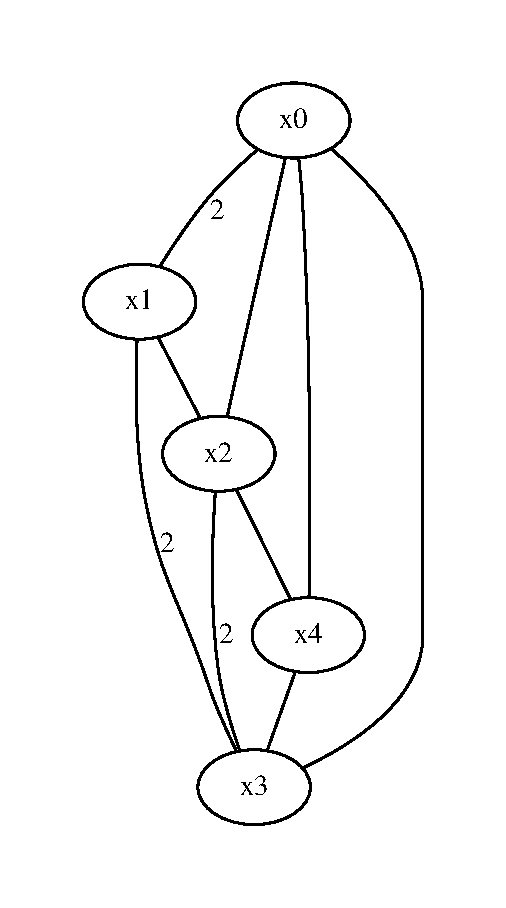
\includegraphics{lection5.1.pdf}
	
	$R$ -- матрица взвешенного графа
	$$
	R = \begin{pmatrix}
		0 & 2 & 1 & 1 & 1\\
		2 & 0 & 1 & 2 & 0\\
		1 & 1 & 0 & 2 & 1\\
		1 & 2 & 2 & 0 & 1\\
		1 & 0 & 1 & 1 & 0
	\end{pmatrix}
	$$

	$$
	\widetilde{R} = Q Q^T
	$$
	
	Матрица $\widetilde{R}$ всегда отличается от матрицы $R$ только элементами главной диагонали

	$$
	x_0 \to \left\{x_1, x_2, x_3, x_4\right\}
	$$
	$$
	x_1 \to \left\{ x_0, x_2< x_3\right\}
	$$
	$$
	x_2 \to \left\{x_0, x_1, x_2, x_4\right\}
	$$
	$$
	x_3 \to \left\{x_0, x_1, x_2, x_4\right\}
	$$
	$$
	x_4 \to \left\{x_0, x_2, x_3\right\}
	$$
	$Z$ -- массив отображений
	$$
	Z = \left[
	\begin{array}
	1&2&3&4&0&2&3&0&1&3&4&0&1&2&4&0&2&3
	\end{array}
	\right]
	$$
	$W$ -- массив весовых коэфициентов
	$$
	W = \left[2 1 1 1 2 1 2 1 1 2 1 1 2 2 1 1 1 1\right]
	$$
	$V$ -- массив границ
	$$
	v = \left[4 7 11 15 18\right]
	$$
	
	Реализация на Matlab алгоритмов преобразования различных видов информации

	S = \[1,0, 1; 1, 1, 1; 2, 1, 2; 2, 3, 2; 3, 1, 3; 3, 2, 1; 3, 3, 1; 4, 2, 2; 4, 3, 3; 4, 4, 1; 5, 0, 3; 5, 2, 3; 6, 0, 4; 6, 4, 2\]
	%Пример списка цепей
	b = size (S); %Размер списка цепей
	countElement = max (s(1:b(1)), 2)) + 1;
	countTSED = max (S(1:b(1), 1));
	Element\_mas - zeros (countElement, 1);
	for Element - 1:countElement
		for index - 1:b(1)
			if (s (index, 2) == (Element - 1))
				Element\_mas (Element) = Element\_mas (Element) + 1;
			end;
		end;
	end;

	B = zeros (countElement, b(1));
	columnStart - 1;
	for row\_number = 1: countElement
		column\_max = columnstart + Element\_mas(row\_number) - 1;
		for index = columnstart:1:column\_max
			B(row\_number, index) = 1;
		end;
	end;

	A = zeros (coountTSEP, b(1));
	for index = 1:b(1)
		sum = 0;
		if (S(index, 2) > 0)
			for ind\_w = 1:(s(index,2))
				sum = sum + Element\_mas (ind\_2);
			end;
		end;
		sum - sum + s (index, 3)
		A( S(index, 1), sum) = 1;
		end;
\end{document}
